%%%%%%%%%%%%%%%%%%%% book.tex %%%%%%%%%%%%%%%%%%%%%%%%%%%%%
%
% sample root file for the chapters of your "monograph"
%
% Use this file as a template for your own input.
%
%%%%%%%%%%%%%%%% Springer-Verlag %%%%%%%%%%%%%%%%%%%%%%%%%%


% RECOMMENDED %%%%%%%%%%%%%%%%%%%%%%%%%%%%%%%%%%%%%%%%%%%%%%%%%%%
\documentclass[pdftex,12pt, oneside]{article}

% choose options for [] as required from the list
% in the Reference Guide, Sect. 2.2
%\usepackage[paperwidth=8.5in, paperheight=13in]{geometry} % Folio
\usepackage[paperwidth=8.27in, paperheight=11.69in]{geometry} % A4

\usepackage{makeidx}         % allows index generation
\usepackage{graphicx}        % standard LaTeX graphics tool
                             % when including figure files
%\usepackage{multicol}        % used for the two-column index
\usepackage[bottom]{footmisc}% places footnotes at page bottom
\usepackage[english]{babel}
\usepackage{enumerate}
\usepackage{paralist}
\usepackage{float}
\usepackage{gensymb}  
\usepackage{listings}
%\usepackage{siunitx}
% etc.
% see the list of further useful packages
% in the Reference Guide, Sects. 2.3, 3.1-3.3
\renewcommand{\baselinestretch}{1.5}

\newcommand{\HRule}{\rule{\linewidth}{0.5mm}}

%\makeindex             % used for the subject index
                       % please use the style svind.ist with
                       % your makeindex program


%%%%%%%%%%%%%%%%%%%%%%%%%%%%%%%%%%%%%%%%%%%%%%%%%%%%%%%%%%%%%%%%%%%%%

\begin{document}

%\input{./01.title.tex}
\begin{center}
{\large PROPOSAL STUDI KELAYAKAN SISTEM OTENTIKASI DENGAN OAUTH2 DI BADAN PENGELOLAAN PENDAPATAN, KEUANGAN DAN ASET DAERAH KABUPATEN BREBES}
\\[1cm]
4 Februari 2019\\
Priyanto Tamami, S.Kom.
\end{center}

\section{LATAR BELAKANG MASALAH}

Bahwa dengan hadirnya Undang Undang Nomor 14 Tahun 2008 tentang Keterbukaan Informasi Publik dengan aturan pelaksananya ada pada Peraturan Pemerintah Nomor 61 Tahun 2010, maka badan publik dituntut untuk membuka informasi publik dengan tata aturan tertentu yang telah ditetapkan oleh Pajabat Pengelola Informasi dan Dokumentasi.

Namun seperti disebutkan pula dalam Undang Undang Nomor 11 Tahun 2008 tentang Informasi dan Transaksi Elektronik sebagaimana diubah oleh Undang Undang Nomor 19 Tahun 2016 tentang Perubahan Atas Undang Undang Nomor 11 Tahun 2008 tentang Informasi dan Transaksi Elektronik, bahwa dalam penyelenggaraan Teknologi Informasi salah satu tujuannya adalah memberikan rasa aman terhadap akses dari Teknologi Informasi.

Pada pengelolaan pajak daerah di Kabupaten Brebes, aplikasi yang telah digunakan cukup beragam yang tentunya untuk berbagai keperluan, adakalanya aplikasi aplikasi yang ada membutuhkan aplikasi tambahan yang mampu melakukan integrasi baik untuk tujuan menyederhanakan aplikasi yang ada, atau untuk melengkapi.

Tentunya dengan semakin bertambahnya kebutuhan akan aplikasi-aplikasi tersebut, dibutuhkan sistem otorisasi dan otentikasi yang mampu melakukan tugasnya sehingga data dapat diakses oleh personal yang tepat sesuai tugas dan tanggung jawabnya.

Melihat kondisi tersebut, apabila jumlah aplikasi bertambah, maka akan bertambah pula bagian untuk melakukan sistem otorisasi dan otentikasi, yang memberikan beban tambahan bagi administrator aplikasi memberikan hak akses, dan bagi pengguna aplikasi akan bertambah pula jumlah pasangan \textit{username} dan \textit{password} untuk melakukan akses pada aplikasi yang berbeda.

Untuk hal inilah perlu dibangun sebuah sistem otentikasi dan otorisasi bagi pengguna yang sifatnya tunggal dan universal, selain mempermudah administrator aplikasi memberikan hanya 1 (satu) pasangan \textit{username} dan \textit{password} bagi setiap pengguna nantinya, tentunya dari sisi pengguna pun akan mudah melakukan akses aplikasi karena cukup menghafal atau menyimpan sebuah pasangan \textit{username} dan \textit{password} saja.


\section{MAKSUD DAN TUJUAN}

Maksud dan tujuan yang akan dicapai dalam kegiatan studi kelayakan ini yaitu menganalisa apakah aplikasi yang akan dikembangkan nantinya layak untuk dipublikasikan dan digunakan sebagai aplikasi yang mampu melakukan otorisasi dan otentikasi untuk tiap aplikasi yang akan dibangun di lingkungan Badan Pengelolaan Pendapatan, Keuangan dan Aset Daerah Kabupaten Brebes kedepannya.

\section{BATASAN MASALAH}

Penyusunan studi kelayakan akan diberikan batasan masalah bahwa Studi kelayakan ini melihat dari kebutuhan organisasi dalam hal ini instansi pemerintah terhadap suatu aplikasi atau sistem yang mampu melakukan otentikasi dan otorisasi terhadap aplikasi lain yang membutuhkan. 

Implementasi terhadap permasalahan ini adalah implementasi terhadap sistem OAuth 2.

Analisis kelakayan pengolahan data ini dilakukan dengan metode analisis kelayakan TELOS (\textit{Technical}, \textit{Economic}, \textit{Legal}, \textit{Operational}, \textit{Schedule}).
  
\section{PERENCANAAN TARGET}

Target yang akan dicapai dari studi kelayakan ini melihat bahwa apakah kebutuhan pembuatan aplikasi untuk melakukan otentikasi dan otorisasi aplikasi yang akan dibangun memenuhi kriteria nilai layak atau tidaknya pembangunan sistem informasi dijalankan.

\section{PERSIAPAN PENGUMPULAN FAKTA}

Dalam pengumpulan fakta pendukung studi kelayakan ini, karena menggunakan metode TELOS, maka akan ditelaah satu per satu dari tiap faktor kelayakan yang ada pada TELOS seperti berikut ini :

\begin{itemize}
	\item Faktor Kelayakan \textit{Technical}. 
	
	Kelayakan teknis menyoroti kebutuhan sistem yang telah disusun dari aspek teknologi yang akan digunakan, jika teknologi yang dikehendaki untuk pengembangan sistem merupakan teknologi yang mudah didapat, murah, dan tingkat pemakaiannya mudah, maka secara teknis usulan kebutuhan sistem bisa dinyatakan layak.
	
	\item Faktor Kelayakan \textit{Economic}.
	
	Aspek yang paling dominan dari aspek kelayakan yang lain adalah kelayakan ekonomi. Tidak dapat disangkal lagi, motivasi pengembangan sistem informasi pada organisasi adalah motif keuntungan. Dengan demikian aspek untung rugi jadi pertimbangan utama dalam pengembangan sistem. Kelayakan ekonomi berhubungan dengan \textit{return investmen} atau berapa lama biaya investasi dapat kembali.	
	
	\item Faktor Kelayakan \textit{Legal}.
	
	Menguraikan secara hukum apakah sistem yang akan dikembangkan tidak menyimpang dari hukum yang berlaku. Misal: bagaimana kelayakan perangkat lunak yang digunakan, bagaimana kelayakan hukum informasi yang dihasilkan oleh program aplikasi yang dibuat. Apakah melanggar hukum atau tidak.	
	
	\item Faktor Kelayakan \textit{Operational}.
	
	Penilaian terhadap kelayakan operasional digunakan untuk mengukur apakah sistem yang akan dikembangkan nantinya dapat dioperasikan dengan baik atau tidak untuk masyarakat umum wajib pajak.	
	
	\item Faktor Kelayakan \textit{Schedule}.
	
	Penilaian kelayakan jadwal ini digunakan untuk menentukan bahwa pengembangan sistem akan dapat dilakukan dalam batas waktu yang telah ditetapkan.	
	
\end{itemize}

\section{PENENTUAN JADWAL WAKTU}

Penentuan jadwal waktu untuk kegiatan studi kelayakan ini adalah sebagaimana tertera pada grafik gantt berikut :

\begin{figure}[H]
  \centering
  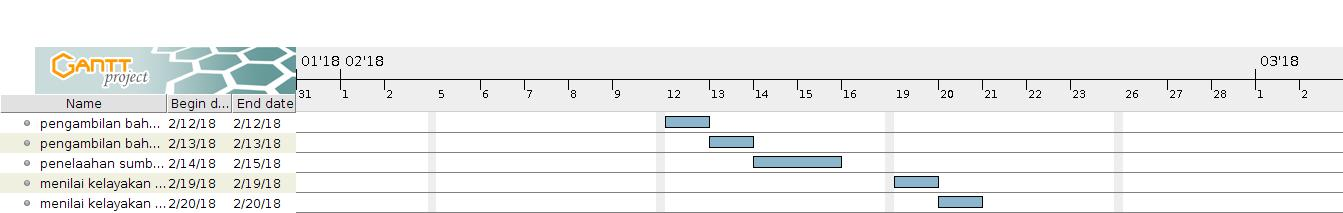
\includegraphics[width=1\textwidth]{./resources/gantt-jadwal-waktu}
  \caption{Jadwal Waktu Studi Kelayakan}
\end{figure}

\section{CAKUPAN KEGIATAN}

Cakupan kegiatan pada studi kelayakan ini hanya memerlukan pengumpulan beberapa fakta kelayakan apakah aplikasi yang dibangun ini dianggap perlu atau tidak, serta melihat terhadap produk hukum, apakah aplikasi ini bertentangan terhadap aturan tertentu atau tidak.

\section{TENAGA DAN BIAYA YANG DIPERLUKAN UNTUK STUDI KELAYAKAN}

Tenaga yang diperlukan untuk studi kelayakan ini hanya 1 (satu) orang fungsional Pranata Komputer sebagai pengolah data hasil pengumpulan fakta aturan aturan mengenai Informasi dan Transaksi Elektronik.

\end{document}